\section{Expansi'on del concepto de 'arbol de an'alisis}

El 'arbol de an'alisis de Heterogenius es el elemento principal de un proceso de demostraci'on, ya que es donde se realizan todas las acciones y es donde se refleja el camino tomado para lograr una demostraci'on exitosa. En su version anterior, el 'arbol de an'alisis solamente presentaba el camino exitoso con lo cual no era capaz de documentar todo el historial del an'alisis realizado. Nos pareci'o importante 'este detalle y necesario poder tambi'en mantener el historial de todas las acciones aplicadas y caminos tomados, ya sean exitosos o no y entre otras cosas reflejar los caminos alternativos.

\begin{figure}[H]
	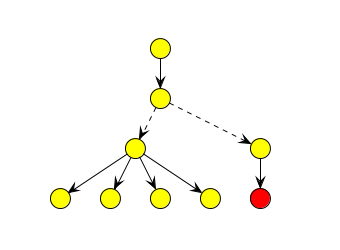
\includegraphics[width=180px]{img/ramas_alternativas_2.png}
	\centering
	\caption{La segunda rama alternativa presenta un contraejemplo. 'Esto indica que existe un contraejemplo para el nodo del cual salen las ramas alternativas.}
\end{figure}

\subsection{Caminos alternativos en una demostraci'on}

Para lograr 'esto se introdujo el concepto de \textit{ramificaci'on alternativa}. En la interface de Heterogenius se representa con lineas punteadas y su significado sem'antico es el de un operador l'ogico \textbf{``o''}. Se corresponde con un camino alternativo en una demostraci'on.

Un nodo con hijos conectados por las ramas alternativas, se entiende que vale si \textit{\textbf{alguna}} de las ramas valen. 'Esto es diferente de la ramificaci'on normal (lineas continuas) que indica que el nodo padre vale si todos sus hijos valen.
 
La principal ventaja de usar caminos alternativos es la de poder documentar todo el an'alisis que se hizo y las decisiones tomadas, incluso las decisiones que no llevaron al cumplimiento del objetivo. Por otro lado tambi'en nos permite experimentar con diferentes formas de probar lo mismo.

\begin{figure}[H]
	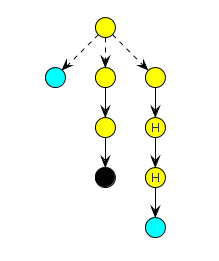
\includegraphics[width=100px]{img/ramas_alternativas.png}
	\centering
	\caption{Tres ramas alternativas: la primera y la 'ultima indican que no se encontr'o ning'un contraejemplo. La segunda rama muestra que se pudo demostrar que el secuente vale, por lo cu'al el secuente del nodo raiz tambi'en vale.}
\end{figure}

TODO: tiene sentido explicar como es la implementacion? los distintos casos, etc??